
\section{Opis planarnog susreta}

\begin{figure}[h!]
    \centering
    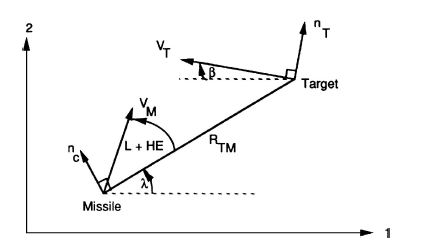
\includegraphics{PNfigure.JPG}
\end{figure}

Udaljenost između mete i projektila u svakom trenutku je data sa:
\begin{equation}
    r(t)=r_T(t)-r_M(t)
\end{equation}
Brzina približavanja projektila meti je data sa: 
\begin{equation}
    v_c=-\dot{r}(t)
\end{equation}

Ugaono ubrzanje mete je dato sa:
\begin{equation}
    \dot{\beta}=\frac{n_T}{v_T}
\end{equation}
Kompnente vektora brzine mete u koordinatnom sistemu vezanom za zemlju su date sa:
\begin{equation}
    v_{T1}=-v_T\cos{\beta}
\end{equation}
\begin{equation}
    v_{T2}=v_T\sin{\beta}
\end{equation}
Slično tome, brzina i ubrzanje projektila su date sa:
\begin{equation}
    \dot{v}_{M1}=a_{M1}
\end{equation}
\begin{equation}
    \dot{v}_{M2}=a_{M2}
\end{equation}
\begin{equation}
    \dot{R}_{M1}=v_{M1}
\end{equation}
\begin{equation}
    \dot{R}_{M2}=v_{M2}
\end{equation}
Ugao \textit{Line of sight} se može izračunati kao:
\begin{equation}
    \lambda = \arctan{\frac{R_{TM2}}{R_{TM1}}}
\end{equation}
Pa je: 
\begin{equation}
    \dot{\lambda}=\frac{R_{TM1}v_{TM2}-R_{TM2}v_{TM1}}{r^2}
\end{equation}
Ugao između vektora pozicije i vektora brzine je dat sa:
\begin{equation}
    L=\arcsin{\frac{v_T\sin{(\beta+\lambda)}}{v_M}}
\end{equation}
Također treba uzeti u obzir da je:
\begin{equation}
    v_{cl}=-\dot{r}=v_M\cos\delta - v_T\cos\theta
\end{equation}
Te da će doći do sudara samo u slučaju da vrijedi: 
\begin{equation}
    v_M\cos\delta > v_T\cos\theta
\end{equation}
Upravljački zakon proporcionalne navigacije je dat sa:
\begin{equation}
    n_C=N'v_c\dot{\lambda}
\end{equation}

%-----------------------------
\section{Izvođenje upravljačkog zakona}
\begin{equation}
    \sin{\lambda}=\frac{y}{r}
\end{equation}
Za male uglove može se koristiti aproksimacija:
\begin{equation}
    \lambda \approx \frac{y}{r}
\end{equation}
, pa je:
\begin{equation}
    \dot{\lambda}(t)=\frac{\dot{y}(t)r(t)-y(t)\dot{r}(t)}{r^2}
\end{equation}
\begin{equation}
    \ddot{\lambda}(t)=\frac{\ddot{y}(t)-2\dot{\lambda}(t)\dot{r}(t)-\lambda(t)\ddot{r}(t)}{r(t)}
\end{equation}
Uvedimo vremenski varijantne koeficijente:
\begin{equation}
    a_1(t)=\frac{\ddot{r}(t)}{r(t)}
\end{equation}
\begin{equation}
    a_2(t)=2\frac{\dot{r}(t)}{r(t)}
\end{equation}
\begin{equation}
    b(t)=\frac{1}{r(t)}
\end{equation}
Pa se dobija diferencijalna jednačina drugog reda sa varijabilnim koeficijenitma:
\begin{equation}
    \ddot{\lambda}(t)=-a_1(t)\lambda-a_2(t)\dot{\lambda}+b(t)\ddot{y}(t)
\end{equation}
Uzimajući u obzir dobija se:
\begin{equation}
    \ddot{y}(t)=-a_M(t)+a_T(t)
\end{equation}
\begin{equation}
    \ddot{\lambda}(t)=-a_1(t)\lambda-a_2(t)\dot{\lambda}-b(t)a_M(t)+b(t)a_T(t)
\end{equation}
Neka je $x_1(t)=\lambda$ i $x_2(t)=\dot{\lambda}$. Tada je susret projektila i mete opisan sljdećim diferencijalnim jednačinama prvog reda.
\begin{equation}
    \dot{x}_1=x_2
    \label{eq:1}
\end{equation}
\begin{equation}
    \dot{x}_2=-a_1(t)x_1-a_2(t)x_2-b(t)u+b(t)f
    \label{eq:2}
\end{equation}
,gdje je uzeto $u=a_M(t)$ i vanjska smetnja $f=a_T(t)$.
Prvo posmatrajmo slučaj kada meta ne ubrzava, tj. kada je $f=0$. Sada se problem proporcionalne navigacije može predstaviti kao:
%\subsection{SubSection Title}
\begin{tcolorbox}
    Pronaći upravljački signal $u$ tako da je sistem opisan jednačinama \ref{eq:1} i \ref{eq:2} asimptotski stabilan u odnosu na $x_2$
\end{tcolorbox}

Shodno tome, uzmimo Lyapunovu funkciju $Q$:
\begin{equation}
    Q=\frac{1}{2}cx_2^2
\end{equation}
Izvod po vremenu duž bilo koje trajektorije je:
\begin{equation}
    \dot{Q}=cx_2(-a_1(t)x_1-a_2(t)x_2-b(t)u(t))
\end{equation}
Sada se vidi da upravljački signal 
\begin{equation}
    u=kx_2=k\dot{\lambda}
    \label{eq:3}
\end{equation}
Stabilizuje sistem dat sa \ref{eq:1} i \ref{eq:2} ako $k$ zadovoljava:
\begin{equation}
    kb(t)+a_2(t)>0
\end{equation}
,odnosno \begin{equation}
    k>-2\dot{r}(t)=2v_{cl}
\end{equation}
Prema tome, uvodeći \textit{efektivni navigacijski odnos} $N$, izraz \ref{eq:3} postaje:
\begin{equation}
    u=Nv_{cl}\dot{\lambda}(t) \quad ,N>2
\end{equation}
čime je potpuno određen zakon vođenja proporcionalne navigacije.
Za trodimenzionalni slučaj se bira kandidat funkcija:
\begin{equation}
    Q=\frac{1}{2}\sum_{s=1}^3d_s\dot{\lambda}_s^2
\end{equation}
, gdje su $d_s$ pozitivni koeficijenti. Analogno se dobija upravljački zakon:
\begin{equation}
    u_s=Nv_{cl}\dot{\lambda}_s \quad ,N>2\ (s=1,2,3)
\end{equation}

\section{Izmjenjena proporcionalna navigacija}
Za mete koje manevrišu i imaju neko normalno ubrzanje, za planarni sustre, izvod Lyapunove kandidat 
funkcije je:
\begin{equation}
    \dot{Q}=cx_2(-a_1(t)x_1-a_2(t)x_2-b(t)u(t)+b(t)f)
\end{equation}
Odakle se zaključuje da je upravljaki signal koji stabilizuje sistem:
\begin{equation}
    u=Nv_{cl}\dot{\lambda}(t)+a_T(t) \quad ,N>2
\end{equation}
\section{Optimalnost zakona proporcionalne navigacije}
Ako je promjena LOS ugla različita od nule, tada se primjenjuje normalno ubrzanje kako bi 
se promjena svela na nulu. U prethodnoj sekciji se proporcionalna navigacija predstavila kao 
problem upravljanja gdje je normalno ubrzanje bilo upravljački signal, a brzina promjene LOS ugla bila varijabla stanja.
Proporcionalna navigacija se može posmatrati kao problem optimalnog upravljanja. Treba pronaći indeks performansi koji 
proporcionalna navigacija minimizira. Ovo predstavlja inverzni problem problem optimalnog upravljanja. Pretpostavimo da 
se projektil približava meti konstantnom brzinom. Ignorišuči dinamiku projektila, vrijedi:
\begin{equation}
    \ddot{y}=-a_M,\ y=r\lambda,\ r(\tau)=v_{cl}\tau
\end{equation}
Također pretpostavlja se da nema kašnjenja u dinamici projektila, tj. da je $a_M = a_{M_c}$.
Definišimo sada ineks performansi:
\begin{equation}
    J=\frac{1}{2}Cy^2(t_f)+\frac{1}{2}\int_0^{t_f}{a_M^2dt}
\end{equation}
Prvi član predstavlja promašaj(miss distance), a drugi predstavlja energiju energiju utrošenu u toku leta. Ideja je pronaći upravljanje
$a_M$ koje minimizira kriterij performanse $J$. Koriteći Bellman-Lyapunov pristup dobija se da je 
optimalno upravljanje dato sa:
\begin{equation}
    a_M(t)=\frac{3\tau}{3/C+\tau ^3}(y(t)+\dot{y}(t)\tau)
\end{equation}
Nulti promašaj se dobija za $C\rightarrow \infty$, pa je optimalno upravljanje dato sa:
\begin{equation}
    a_M(t)=\frac{3}{\tau ^2}(y(t)+\dot{y}(t)\tau)
\end{equation}
Uzimajući u obzir da je:
\begin{equation}
    \dot{\lambda} = \frac{\dot{y}(t)r(t)-y(t)\dot{t}(t)}{r^2}=\frac{\dot{y}(t)\tau + y(t)}{r}
\end{equation}
jer je, $r=v_{cl}\tau$, dobija se:
\begin{equation}
    a_M(t)=3v_{cl}\dot{\lambda}
\end{equation}
Ovo znači da pod uvedenim pretpostavkama, proporcionalna navigacija minimizira kriterij performanse
$J$ i izbor efektivnog navigacijskog odnosa $N=3$ garantuje da nulti promašaj. 
%-----------------------
\section{Linearizacija}
\begin{figure}[h!]
    \centering
    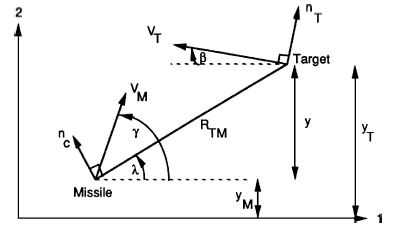
\includegraphics{linearPN.JPG}
    \caption{Linearizacija jednačina proporcionalne navigacije}
    \label{fig:linear}
\end{figure}

Linearizacija se može lahko izvršiti ako se definišu nove veličine koje su prikazane na slici \ref{fig:linear}.
Relativno ubrzanje se može odrediti sa slike i iznosi:
\begin{equation}
    \ddot{y}=n_T\cos\beta-n_c\cos\lambda
\end{equation}
Ako su uglovi leta mali, tada vrijedi:
\begin{equation}
    \ddot{y}=n_T-n_c
\end{equation}
Slično tako vrijedi:
\begin{equation}
    \lambda = \frac{y}{r}
\end{equation}
Za čeoni slučaj vrijedi:
\begin{equation}
    v_{cl}=v_M+v_t
\end{equation}
Za potjeru vrijedi:
\begin{equation}
    v_{cl}=v_M-v_t
\end{equation}
Sada se može linearizirati i jednačina za udaljenost:
\begin{equation}
    r(t)=v_{cl}(t_F-t)
\end{equation}
gdje je $t_F$ ukupno vrijeme leta.\\
Definišimo i veličinu \textit{time to go} $t_{go}$:
\begin{equation}
    t_{go}=t_F-t
\end{equation}
Linearizirani promašaj se definisše kao udaljenost mete i projektila na kraju leta, ili:
\begin{equation}
    Miss=y(t_f)
\end{equation}

\section{Zero effort miss}
Ranije je pokazano da vrijedi:
\begin{equation}
    \dot{\lambda}(t)=\frac{\dot{y}(t)r(t)+y(t)v_{cl}}{r^2}
\end{equation}
Kako vrijedi $r=v_{cl}t_{go}$, tada se dobija:
\begin{equation}
    \dot{\lambda}(t)=\frac{\dot{y}(t)t_{go}+y(t)}{v_{cl}t_{go}^2}
\end{equation}
Definišimo sada veličinu \textit{Zero effort miss}, koja predstavlja buduće relativno rastojanje projektila i mete:
\begin{equation}
    ZEM=\dot{y}(t)t_{go}+y(t)
\end{equation}
pa se dobija:
\begin{equation}
    \dot{\lambda}(t)=\frac{ZEM}{v_{cl}t_{go}^2}
\end{equation}
Ako se pretpstavi da će se pod uticajem ubrzanja $a_c$ postići sudar, $ZEM$ se može smatrati 
budućom tačkom susreta, pa se zakon vođenja proprcionalne navigacije može iskazati kao:
\begin{equation}
    a_c(t)=N\frac{ZEM}{t_{go}^2}
\end{equation}
Sada se vidi da je normalno ubrzanje projektila direktno proprorcionalnu $ZEM$-u i inverzno proporcionalno
kvadratu preostalom vremenu leta, što znači da se generiše veće ubrzanje što je susret bliži.
Pošto se $ZEM$ posmatra kao buduća tačka susreta, koja se računa na osnovu znanja ili pretpostavki 
budučeg kretanja mete, PN vođenje se smatra prediktivnim. $ZEM$ je koristan jer se može izračunati 
mnoštvom metoda uključujući i on-line numeričku integraciju nelinearnih diferencijalnih jednačina projektila 
i mete. 

\begin{figure}
    \centering
    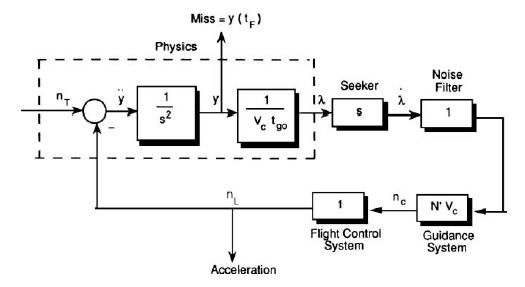
\includegraphics{homingLoop.JPG}
    \label{fig:homing}
\end{figure}